\section{准备工作}

搭建分布式集群环境需要准备几台互联的计算机,并且在每台计算机上都安装好分布式环境以及DETRIA软件运行需要的环境(RELAP5等)。

\subsection{硬件准备}
\begin{enumerate}
    \item 若干台计算机节点
    \item 连接工具:交换机、网线、路由器
\end{enumerate}

\subsection{安装操作系统}
Windows Server 2019是由微软(Microsoft)官方推出的最新版服务器版操作系统,该系统基于Win Server 2016开发而来,后者是微软迄今为止普及速度最快的服务器系统。WinServer 2019 与 Win10 同宗同源,提供了 GUI 界面,包含了大量服务器相关新特性,也是微软提供长达十年技术支持(简称 LTSC)的新一代产品。Windows Server 2019主要用于 VPS 或 服务器上,可用于架设网站或者提供各类网络服务。

安装Windows Server 2019的主要步骤:
\begin{enumerate}
    \item 在\href{https://www.microsoft.com/en-us/evalcenter/evaluate-windows-server-2019}{Microsoft官网}下载ISO镜像文件
    \item 使用安装介质(USB闪存驱动器、DVD等)安装系统
    \item 设置密码(每台计算机密码尽量设置相同),激活系统
\end{enumerate}

\subsection{记录节点IP地址}
安装好操作系统后,打开命令提示符,输入$ ifconfig $命令查看计算机ip,查看计算机ip地址,如\ref{ipconfig查看IP地址}所示。
\begin{figure}[h]
    \centering
    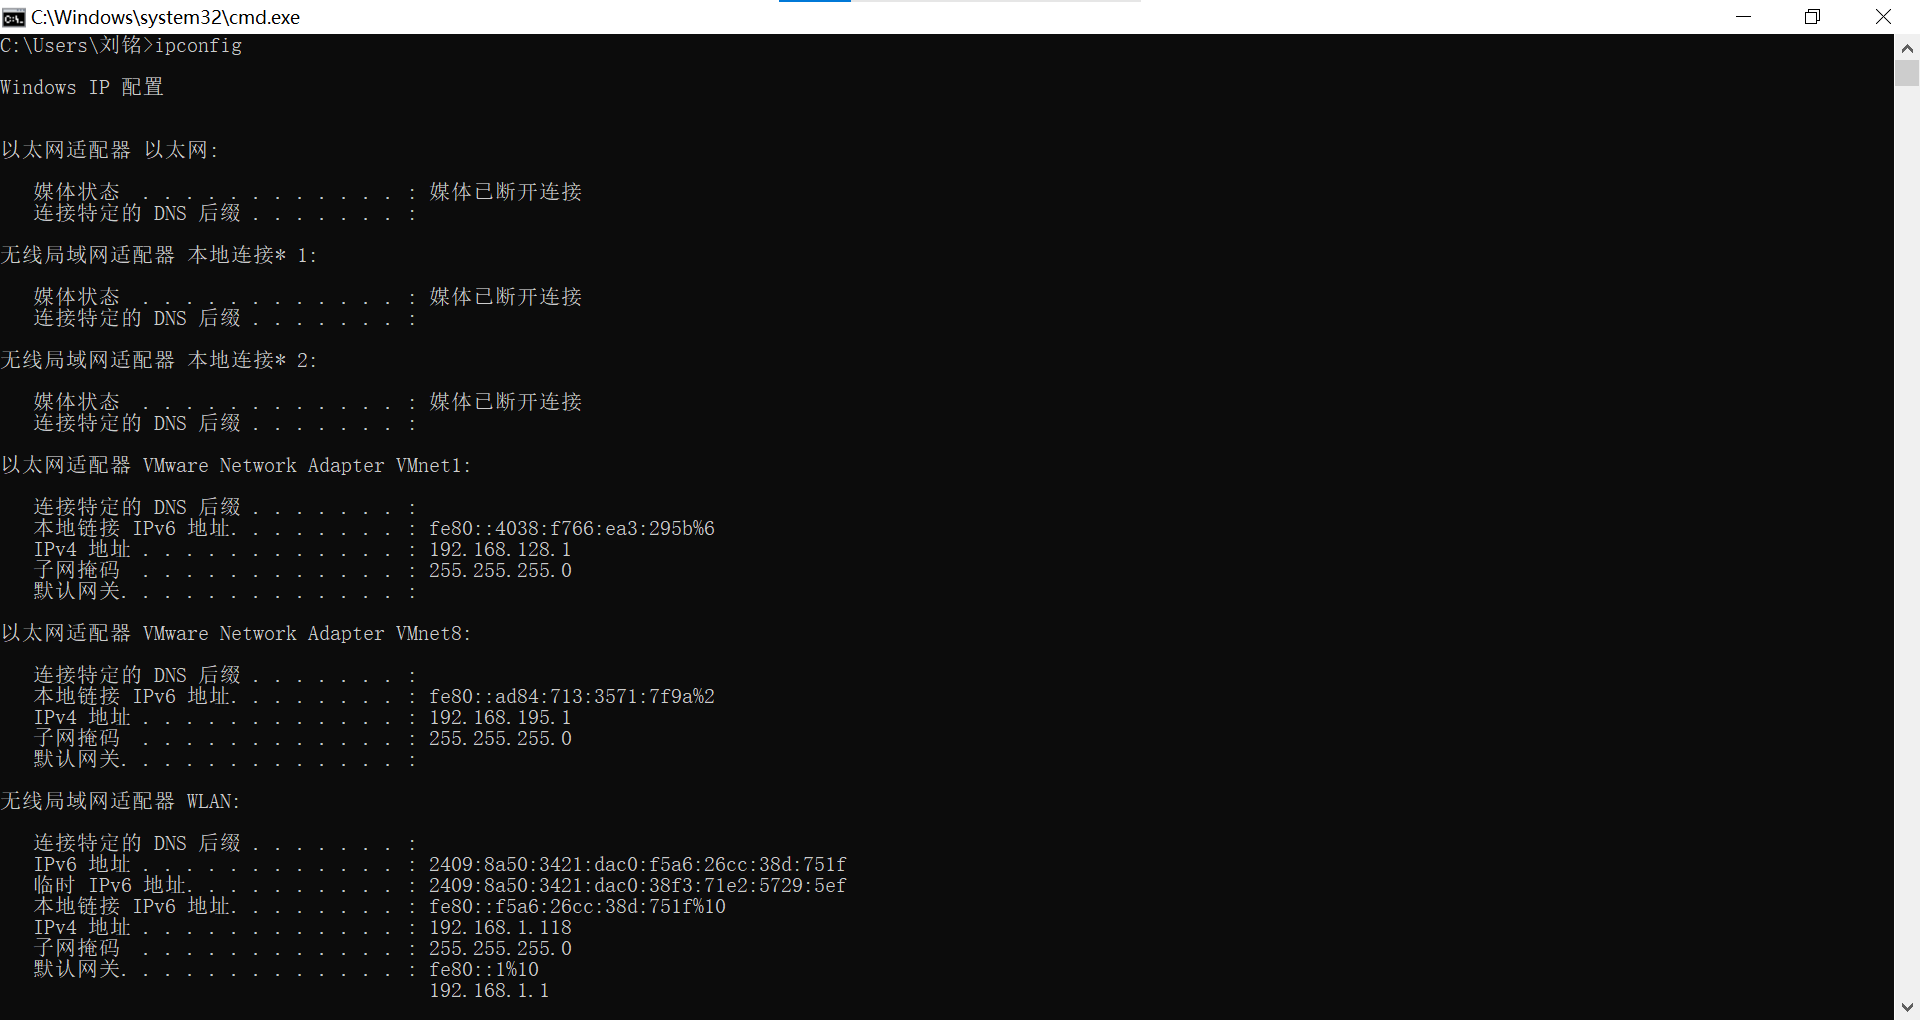
\includegraphics[width=1.0\textwidth]{ipconfig.png}
    \caption{ipconfig查看IP地址}
    \label{ipconfig查看IP地址}
\end{figure}